% Atividade assíncrona — Lugar das raízes (Trabalho de Projeto de Compensadores)
% Disciplina: Controle Aplicado à Computação — UFSC
% Compilar: pdflatex (duas vezes, se usar hyperref)

\documentclass[11pt,a4paper]{article}

\usepackage[utf8]{inputenc}
\usepackage[T1]{fontenc}
\usepackage[brazil]{babel}
\usepackage{geometry}
\geometry{margin=2.5cm}
\usepackage{amsmath, amssymb}
\usepackage{graphicx}
\usepackage{caption}
\captionsetup{font=small, labelfont=bf}
\usepackage{hyperref}
\usepackage{enumitem}

\setlist[itemize]{noitemsep, topsep=4pt}
\setlist[enumerate]{noitemsep, topsep=4pt}

\hypersetup{
  colorlinks=true,
  linkcolor=blue,
  urlcolor=blue,
}

\title{\textbf{Atividade: Lugar das raízes}}
\author{
  Igor de Matos da Rosa\\
  Matrícula: 20103930\\[0.5em]
  \textit{Controle Aplicado à Computação}\\
  Universidade Federal de Santa Catarina (UFSC)
}
\date{Araranguá, 2026}

\begin{document}

\maketitle

% ---------------------------------------------------------------------------
\section*{Questão 1 --- Exercício B.6.14}
% ---------------------------------------------------------------------------

\subsection*{Enunciado}

Parto do sistema em realimentação unitária negativa com
\begin{equation}
  G(s)=\frac{K}{s(s^2+4s+5)} .
\end{equation}
\textbf{Preciso determinar} o lugar das raízes (conceitualmente), o ganho $K$ tal que o coeficiente de amortecimento dos polos dominantes em malha fechada seja $\zeta=0{,}5$, \textbf{obter todos} os polos em malha fechada para esse $K$ e \textbf{comentar} a resposta ao degrau unitário.

\subsection*{Equação característica}

Considerando $H(s)=1$, escrevo a malha fechada como $T(s)=\dfrac{G(s)}{1+G(s)}$. A condição $1+G(s)=0$ equivale a
\begin{equation}
  s(s^2+4s+5)+K=0
  \quad\Longrightarrow\quad
  s^3+4s^2+5s+K=0 .
\end{equation}

\subsection*{Polos de malha aberta}

As raízes de $s(s^2+4s+5)=0$ fornecem os polos de $G(s)$:
\begin{itemize}
  \item $s=0$;
  \item $s=-2\pm j$, pois $s^2+4s+5=0 \Rightarrow s=\dfrac{-4\pm\sqrt{16-20}}{2}=-2\pm j$.
\end{itemize}
\textbf{São três polos} e \textbf{nenhum zero finito}; por isso imagino o lugar das raízes com três ramos indo ao infinito.

\subsection*{Projeto para $\zeta=0{,}5$ (semi-plano superior)}

Para um par complexo na forma usual $s=-\zeta\omega_n \pm j\omega_n\sqrt{1-\zeta^2}$, uso que o ângulo $\phi$ medido a partir do semi-eixo real negativo até o vetor do polo satisfaz $\cos\phi=\zeta$. Para $\zeta=0{,}5$:
\begin{equation}
  \phi=\arccos(0{,}5)=\frac{\pi}{3}\,\mathrm{rad}\;(60^\circ).
\end{equation}
Defino $\theta$ como o ângulo a partir do eixo real positivo,
\begin{equation}
  \theta=\pi-\phi=\frac{2\pi}{3}.
\end{equation}
Então procuro os polos desejados no semi-plano superior sobre a semi-reta
\begin{equation}
  s=r\,e^{j2\pi/3},\qquad r>0 .
\end{equation}

Substituindo $s=r\,e^{j2\pi/3}$ na expressão $s^3+4s^2+5s$ e impondo parte imaginária nula (porque $K\in\mathbb{R}$), cheguei a $r=\dfrac{5}{4}$ e
\begin{equation}
  K=\frac{275}{64}=4{,}296875 .
\end{equation}
Os dois polos complexos ficam então em
\begin{equation}
  s=-\frac{5}{8}\pm j\frac{5\sqrt{3}}{8}
  \approx -0{,}625 \pm j\,1{,}082532 .
\end{equation}

\subsection*{Todos os polos em malha fechada}

Para $K=\dfrac{275}{64}$, trabalho com $s^3+4s^2+5s+\dfrac{275}{64}=0$ e obtenho as raízes:
\begin{itemize}
  \item $s_1=-2{,}75$ (polo real);
  \item $s_{2,3}=-0{,}625 \pm j\,1{,}082532$ (par complexo com $\zeta=0{,}5$ e $\omega_n=|s|=1{,}25\,\mathrm{rad/s}$).
\end{itemize}

Interpretando as posições: o polo real fica mais à esquerda e o par complexo mais próximo do eixo imaginário, de modo que esse par tende a dominar o transitório que observo na resposta ao degrau.

\subsection*{Resposta ao degrau}

A malha fechada resulta tipo~1 (integrador na malha aberta); para degrau unitário, espero erro estacionário de posição nulo e $y(\infty)=1$.

\begin{figure}[htbp]
  \centering
  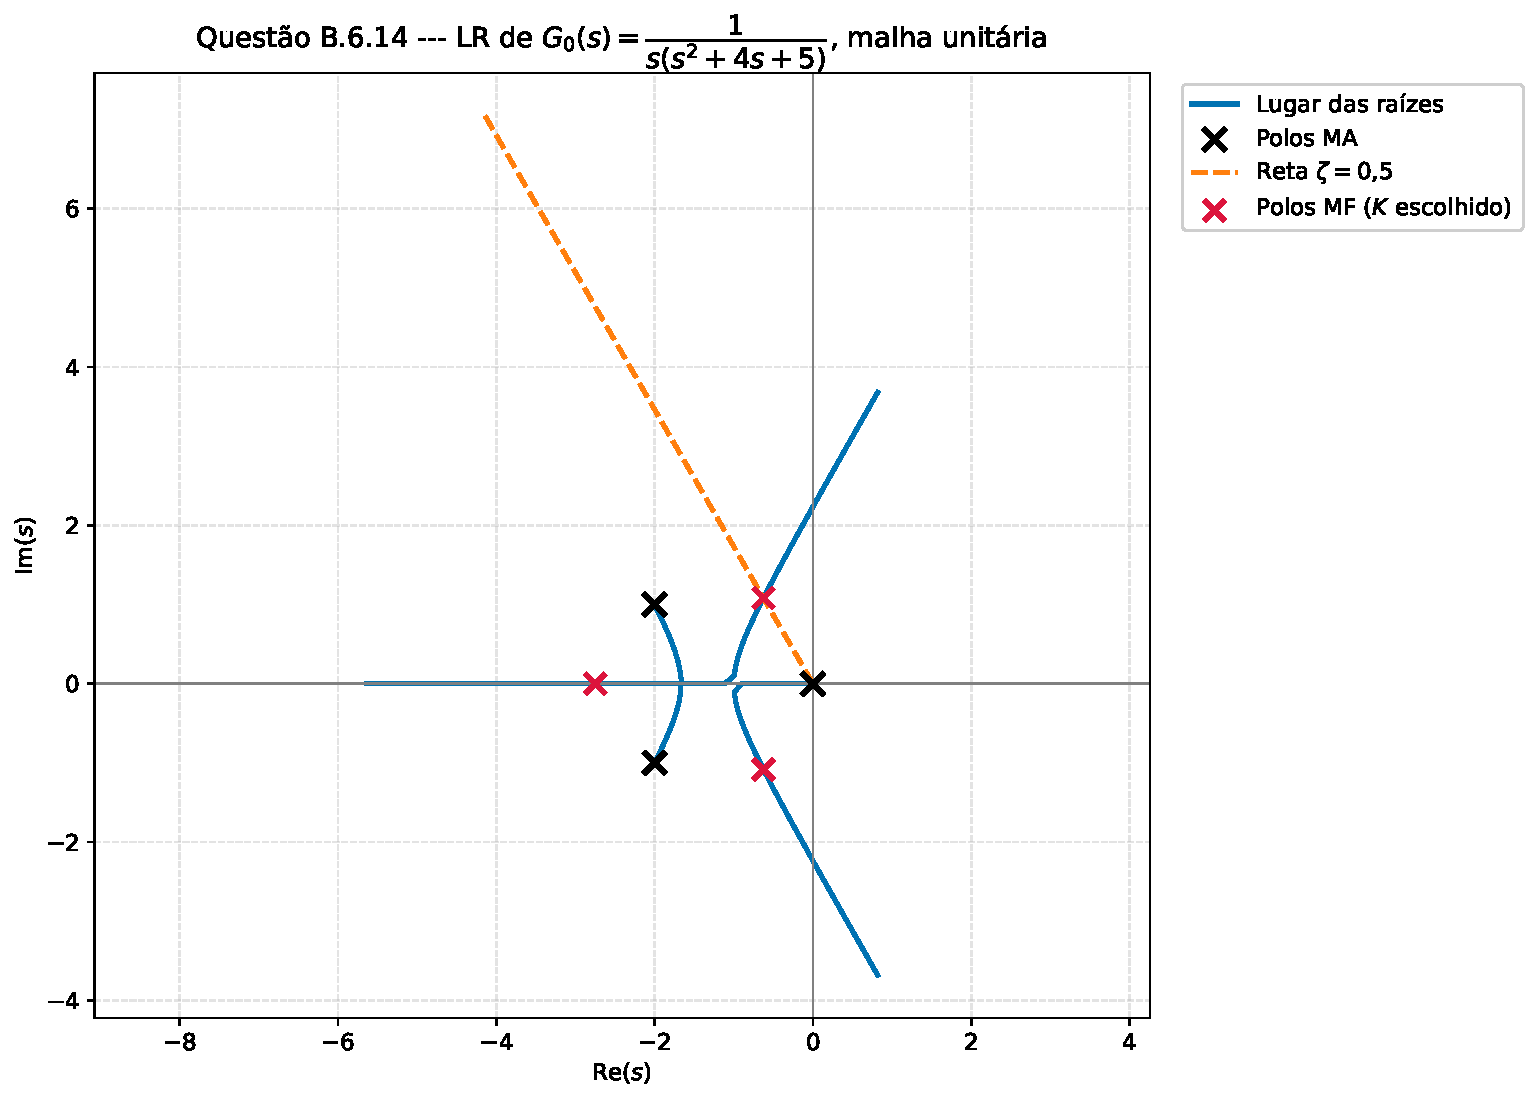
\includegraphics[width=\linewidth]{fig_b614_lugar_raizes.pdf}
  \caption{B.6.14 --- Lugar das raízes de $G_0(s)=\dfrac{1}{s(s^2+4s+5)}$ com malha unitária; reta de $\zeta=0{,}5$; polos de malha fechada para $K=275/64$.}
  \label{fig:b614rl}
\end{figure}

\begin{figure}[htbp]
  \centering
  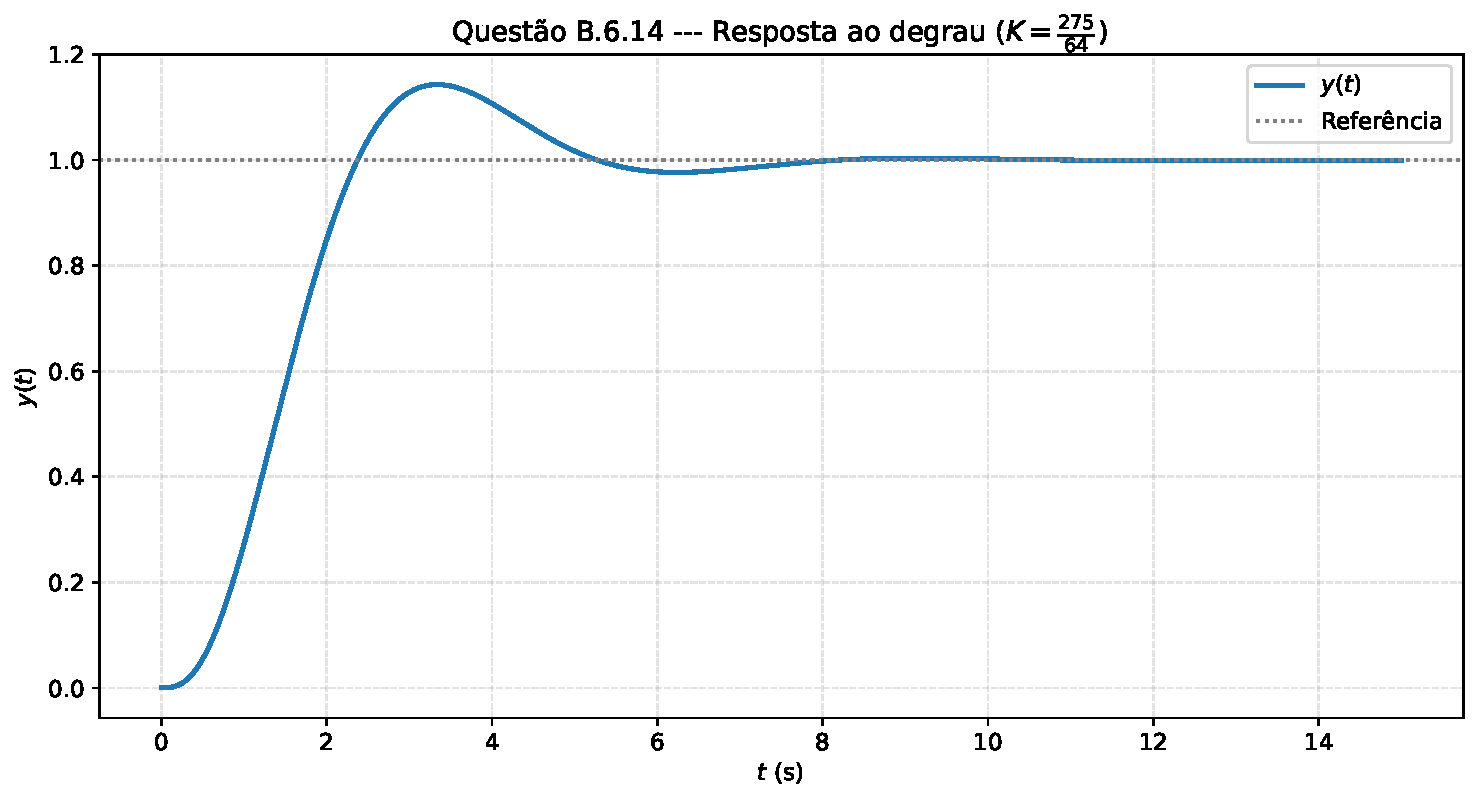
\includegraphics[width=0.92\linewidth]{fig_b614_degrau.pdf}
  \caption{B.6.14 --- Resposta ao degrau unitário da malha fechada com $K=\dfrac{275}{64}$.}
  \label{fig:b614step}
\end{figure}

% ---------------------------------------------------------------------------
\section*{Questão 2 --- Exercício B.6.15}
% ---------------------------------------------------------------------------

\subsection*{Enunciado}

\textbf{Preciso determinar} $K$, $T_1$ e $T_2$ para o sistema em realimentação unitária negativa com
\begin{equation}
  G(s)=\left[K\frac{T_1s+1}{T_2s+1}\right]\frac{10}{s(s+1)} ,
\end{equation}
de forma que os polos dominantes em malha fechada tenham amortecimento $\zeta=0{,}5$ e frequência natural não amortecida $\omega_n=3\,\mathrm{rad/s}$.

\subsection*{Polos dominantes desejados}

\begin{equation}
  s=-\zeta\omega_n \pm j\omega_n\sqrt{1-\zeta^2}
  = -1{,}5 \pm j\frac{3\sqrt{3}}{2}
  \approx -1{,}5 \pm j\,2{,}598076 .
\end{equation}
Escrevendo o polinômio quadrático associado:
\begin{equation}
  s^2+2\zeta\omega_n s+\omega_n^2 = s^2+3s+9 .
\end{equation}

\subsection*{Equação característica}

Partindo de $1+G(s)=0$ e multiplicando pelo denominador comum:
\begin{equation}
  (T_2s+1)\,s(s+1)+10K(T_1s+1)=0 ,
\end{equation}
isto é,
\begin{equation}
  T_2s^3+(T_2+1)s^2+(1+10KT_1)s+10K=0 .
  \label{eq:car615}
\end{equation}

Como o sistema é de terceira ordem, ao fixar só o par dominante ainda sobra um grau de liberdade (o terceiro polo real $s=-p$). Por isso imagino, em princípio, uma \textbf{família} de ternos $(K,T_1,T_2)$ até que eu faça uma escolha extra que fecha a solução.

\subsection*{Casamento com $(s^2+3s+9)(s+p)$}

Expandindo,
\begin{equation}
  (s^2+3s+9)(s+p)=s^3+(p+3)s^2+(3p+9)s+9p .
\end{equation}
Comparando com a expressão~\eqref{eq:car615} depois de dividir por $T_2\neq 0$, cheguei a
\begin{align}
  \frac{T_2+1}{T_2} &= p+2\zeta\omega_n ,\\
  10K &= T_2\,\omega_n^2 p ,\\
  1+10KT_1 &= T_2\,(2\zeta\omega_n p+\omega_n^2).
\end{align}
Para $\zeta=0{,}5$ e $\omega_n=3$, uso $2\zeta\omega_n=3$, logo
\begin{equation}
  p=\frac{T_2+1}{T_2}-3=\frac{1}{T_2}-2 .
\end{equation}

\subsection*{Solução usual (cancelamento em $s=-1$)}

A planta tem polo em $s=-1$. Escolhendo $T_1=1$, posiciono o zero do compensador em $-1/T_1=-1$ e cancelo esse polo na malha aberta.

Substituindo $T_1=1$ e resolvendo o sistema fechado para $\zeta=0{,}5$ e $\omega_n=3$, cheguei à solução única
\begin{equation}
  \boxed{T_1=1,\qquad T_2=\frac{1}{3},\qquad K=\frac{3}{10}=0{,}3.}
\end{equation}

Os polos em malha fechada que obtive são $-1{,}5\pm j\,3\sqrt{3}/2$ e $s=-1$. Observo que, como $|{-}1|<|{-}1{,}5|$, o modo exponencial associado a $s=-1$ é mais lento que o envelope do par complexo; num critério estrito de dominância por parte real, esse polo pode influenciar o transitório. Se for necessário acelerar o terceiro modo de forma que $p>\zeta\omega_n=1{,}5$, reduzo $T_2$ dentro da família de soluções (por exemplo, $T_2=0{,}25$).

\subsection*{Resposta ao degrau e lugar das raízes}

Com $T_1=1$, $T_2=1/3$ e $K=0{,}3$, verifiquei que a malha fechada segue tipo~1 com ganho DC unitário para rastrear o degrau.

\begin{figure}[htbp]
  \centering
  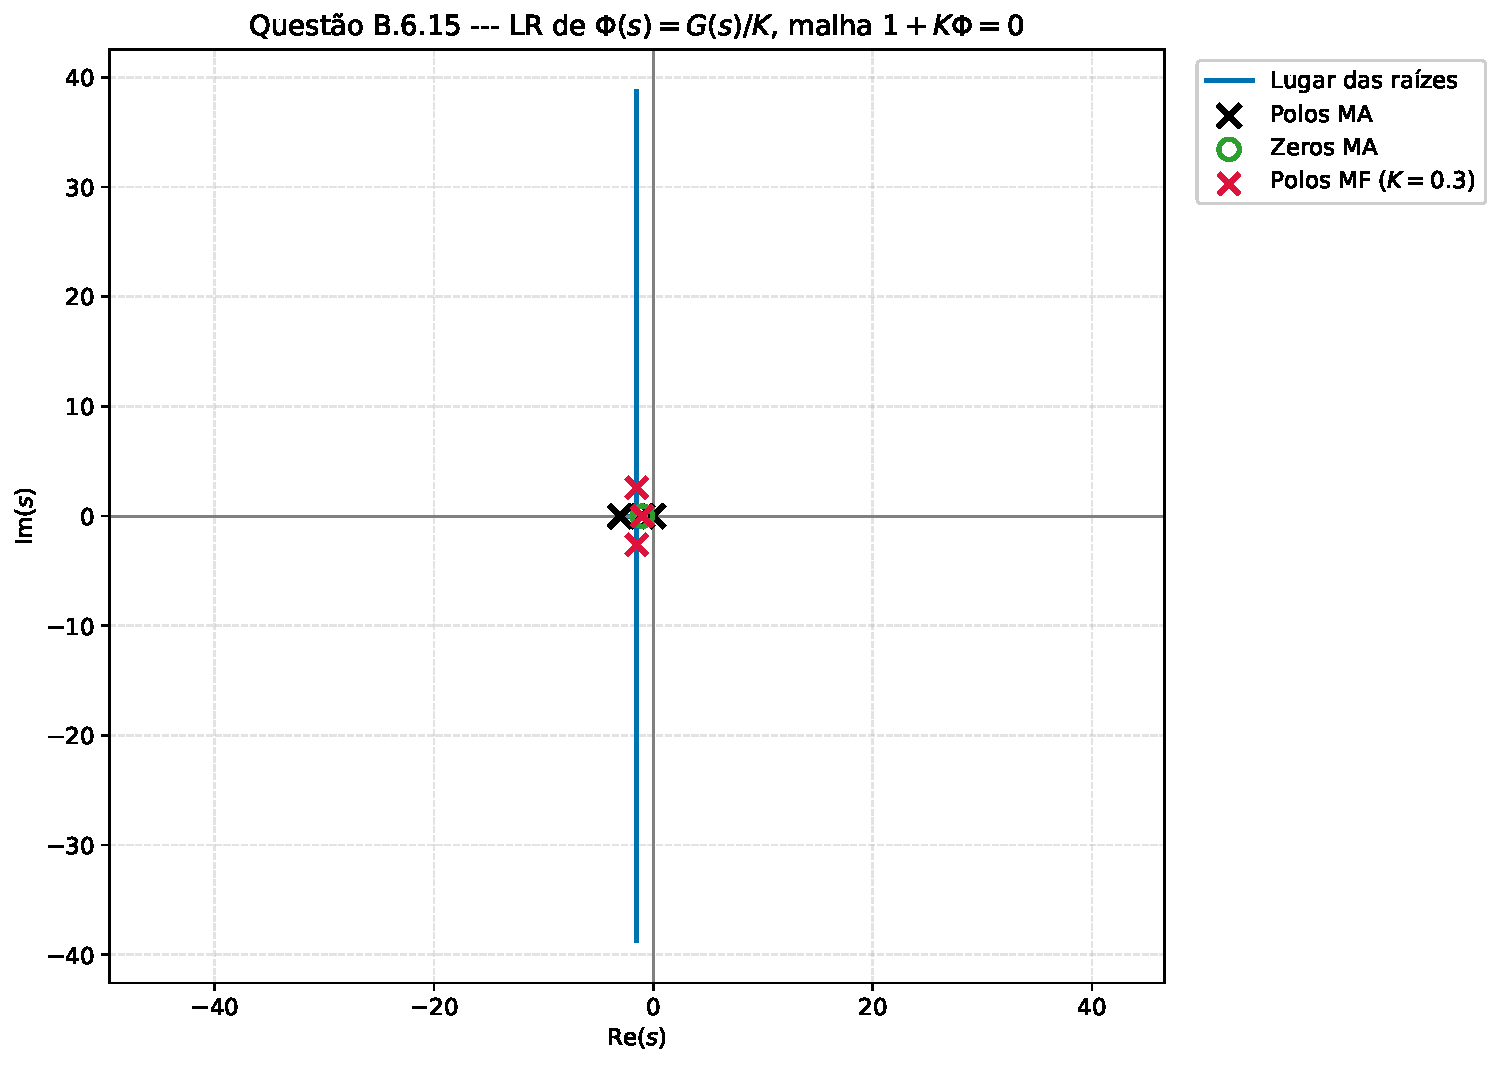
\includegraphics[width=\linewidth]{fig_b615_lugar_raizes.pdf}
  \caption{B.6.15 --- Lugar das raízes da função $\Phi(s)=G(s)/K$ tal que $1+K\Phi(s)=0$ equivale à malha original; polos e zeros de malha aberta e polos de malha fechada para $K=0{,}3$, $T_1=1$, $T_2=1/3$.}
  \label{fig:b615rl}
\end{figure}

\begin{figure}[htbp]
  \centering
  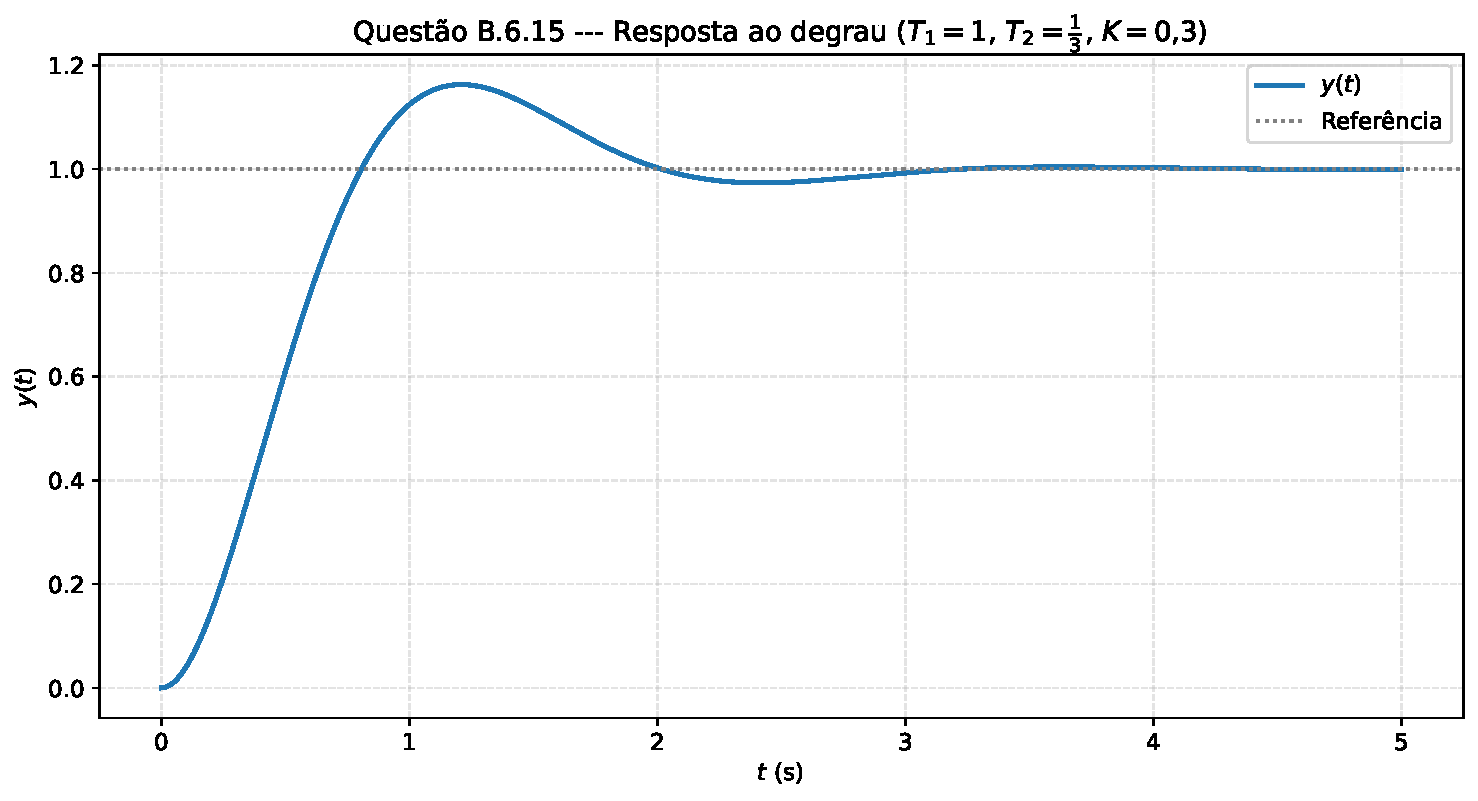
\includegraphics[width=0.92\linewidth]{fig_b615_degrau.pdf}
  \caption{B.6.15 --- Resposta ao degrau unitário com $T_1=1$, $T_2=\dfrac{1}{3}$, $K=\dfrac{3}{10}$.}
  \label{fig:b615step}
\end{figure}

% ---------------------------------------------------------------------------
\section*{Questão 3 --- Exercício B.6.18}
% ---------------------------------------------------------------------------

\subsection*{Enunciado}

\textbf{Preciso projetar} um compensador de avanço de fase para o sistema em realimentação unitária negativa com planta $G_p(s)=1/s^2$ e compensador
\begin{equation}
  G_c(s)=K\,\frac{s+z}{s+p},\qquad p>z>0,
\end{equation}
de forma que os polos dominantes em malha fechada fiquem em $s=-1\pm j1$.

\subsection*{Polos dominantes desejados}

O par complexo impõe
\begin{equation}
  \omega_n=\sqrt{2}\,\mathrm{rad/s},\qquad
  \zeta=\frac{1}{\sqrt{2}}\approx 0{,}707,
\end{equation}
e o fator quadrático associado $s^2+2s+2$.

\subsection*{Equação característica}

Com $H(s)=1$, a malha aberta é
\begin{equation}
  G(s)=G_c(s)G_p(s)=\frac{K(s+z)}{s^2(s+p)}.
\end{equation}
A condição $1+G(s)=0$ fornece
\begin{equation}
  s^3+ps^2+Ks+Kz=0.
  \label{eq:car618}
\end{equation}

\subsection*{Casamento com um terceiro polo real}

Como o sistema é de terceira ordem, além do par em $-1\pm j1$ escolho um polo real em $s=-c$ ($c>0$) e imponho
\begin{equation}
  (s^2+2s+2)(s+c)=s^3+(c+2)s^2+(2c+2)s+2c.
\end{equation}
Comparando com~\eqref{eq:car618}:
\begin{equation}
  p=c+2,\qquad K=2c+2,\qquad z=\frac{c}{c+1}.
\end{equation}
Para avanço de fase exijo $p>z$, satisfeito para todo $c>0$. Para dominância do par complexo, posiciono o polo real bem à esquerda; adoto $c=5$ (polo em $-5$).

\subsection*{Parâmetros do compensador}

\begin{equation}
  \boxed{z=\frac{5}{6},\qquad p=7,\qquad K=12,}
\end{equation}
isto é,
\begin{equation}
  G_c(s)=12\,\frac{s+\dfrac{5}{6}}{s+7}.
\end{equation}
Os polos em malha fechada que obtive são $-1\pm j1$ e $-5$.

\subsection*{Condição de ângulo}

No ponto $s_d=-1+j1$, a planta contribui $\angle(1/s^2)=90^\circ$. O compensador deve somar $90^\circ$ para satisfazer a condição de fase do lugar das raízes:
\begin{equation}
  \angle(s_d+z)-\angle(s_d+p)=90^\circ.
\end{equation}
Com $z=5/6$ e $p=7$ verifiquei essa condição; o ganho $K$ segue da condição de módulo $|G(s_d)|=1$.

\subsection*{Resposta ao degrau e lugar das raízes}

\begin{figure}[htbp]
  \centering
  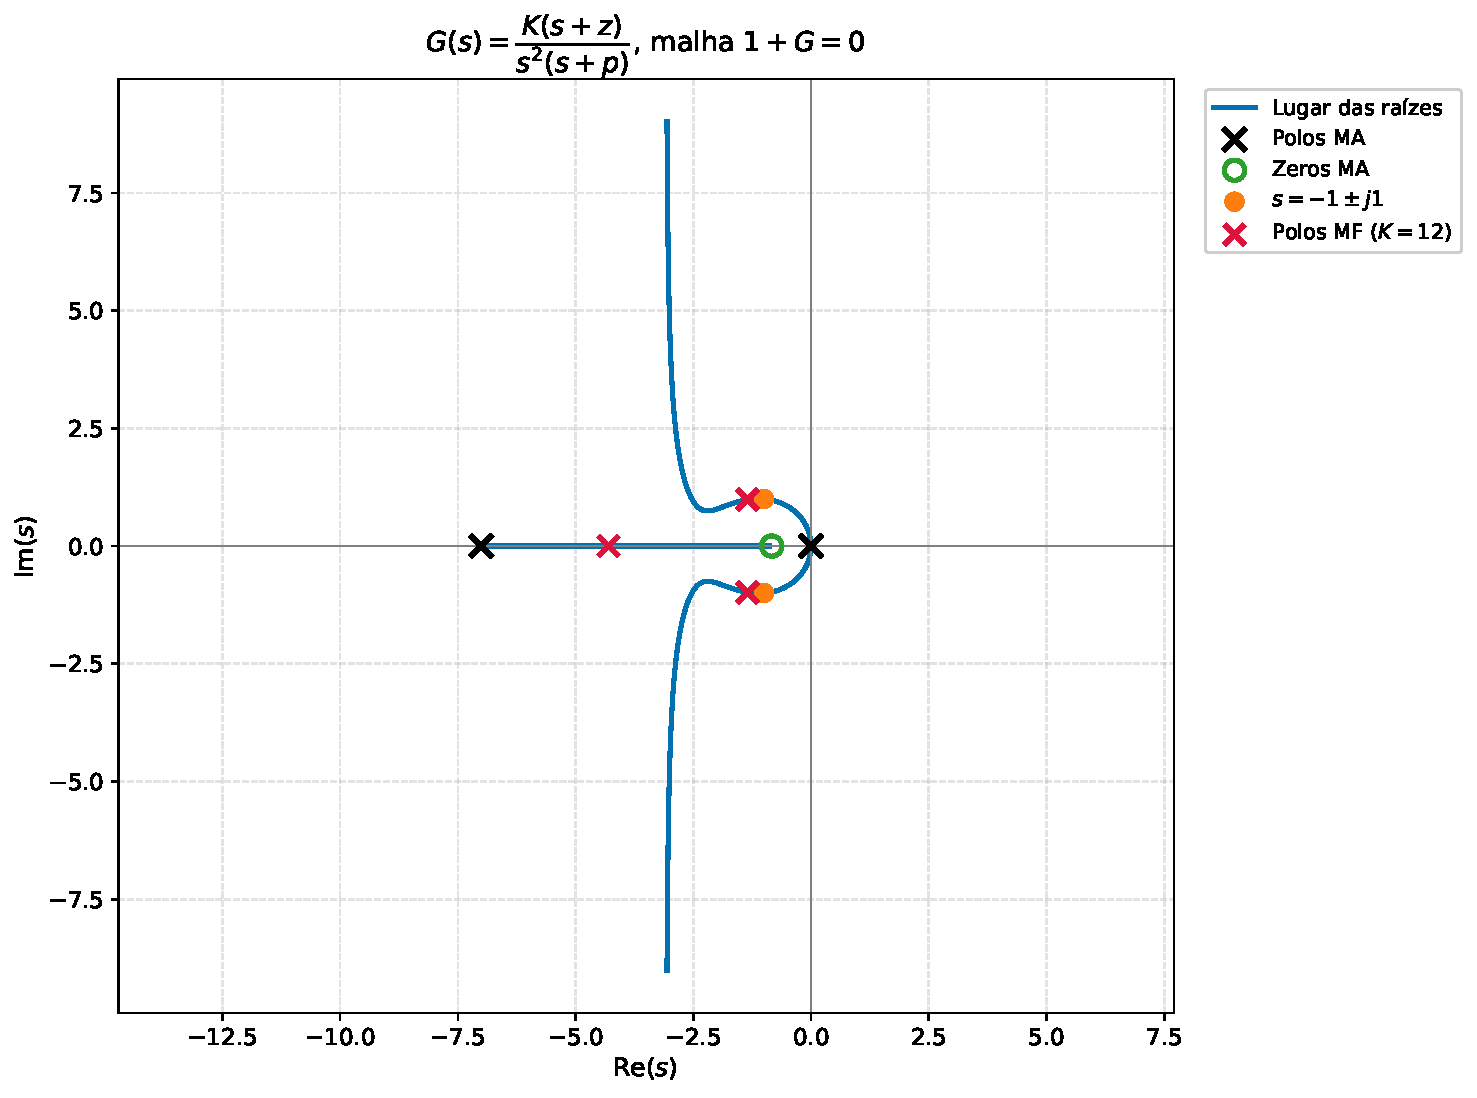
\includegraphics[width=\linewidth]{fig_b618_lugar_raizes.pdf}
  \caption{B.6.18 --- Lugar das raízes de $G(s)=\dfrac{K(s+z)}{s^2(s+p)}$; polos desejados e polos de malha fechada para $K=12$, $z=5/6$, $p=7$.}
  \label{fig:b618rl}
\end{figure}

\begin{figure}[htbp]
  \centering
  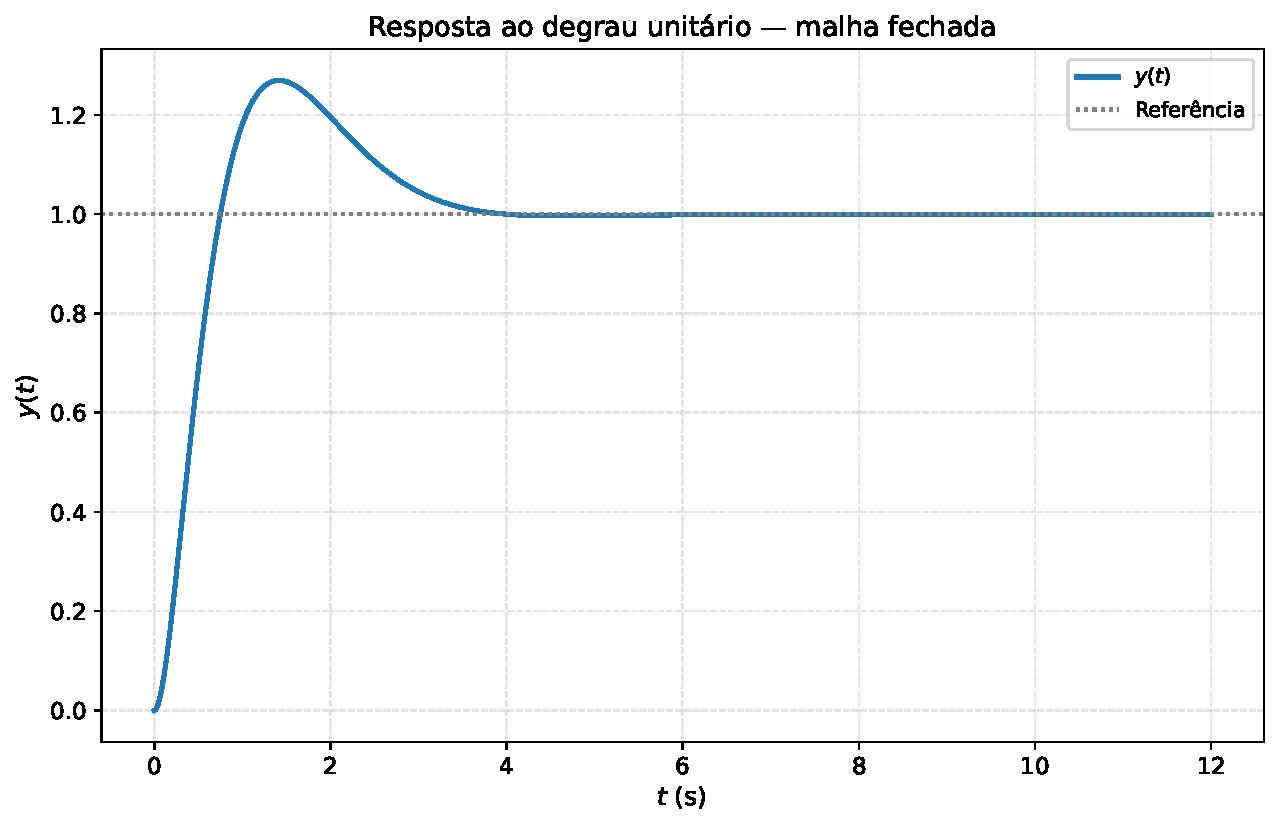
\includegraphics[width=0.92\linewidth]{fig_b618_degrau.pdf}
  \caption{B.6.18 --- Resposta ao degrau unitário da malha fechada compensada.}
  \label{fig:b618step}
\end{figure}

% ---------------------------------------------------------------------------
\section*{Questão 4 --- Exercício B.6.20}
% ---------------------------------------------------------------------------

\subsection*{Enunciado}

Considero o sistema de posicionamento angular com malha unitária e
\begin{equation}
  G(s)=\frac{820}{s(s+10)(s+20)}.
\end{equation}
Os polos dominantes atuais estão em $s=-3{,}60\pm j4{,}80$, com $\zeta=0{,}6$ e $K_v=4{,}1\,\mathrm{s}^{-1}$. Para rampa de $360^\circ/\mathrm{s}$,
\begin{equation}
  e_v=\frac{\theta_i}{K_v}=\frac{360}{4{,}1}\approx 87{,}8^\circ.
\end{equation}
\textbf{Preciso} reduzir $e_v$ para um décimo do valor atual ($K_v=41\,\mathrm{s}^{-1}$), mantendo $\zeta\approx 0{,}6$, por meio de um compensador de atraso de fase.

\subsection*{Sistema sem compensação}

Do par dominante,
\begin{equation}
  \omega_n=6\,\mathrm{rad/s},\qquad \zeta=\frac{3{,}6}{6}=0{,}6.
\end{equation}
A constante de velocidade estática é
\begin{equation}
  K_v=\lim_{s\to 0}sG(s)=\frac{820}{10\cdot 20}=4{,}1\,\mathrm{s}^{-1}.
\end{equation}

\subsection*{Fator $\beta$ e modelo do atraso}

Para dividir o erro em rampa por $10$:
\begin{equation}
  \beta=\frac{K_{v,\mathrm{desejado}}}{K_{v,\mathrm{atual}}}=\frac{41}{4{,}1}=10.
\end{equation}
Utilizo o compensador de Ogata (Eq.~6-19):
\begin{equation}
  G_c(s)=\hat K_c\,\beta\,\frac{Ts+1}{\beta Ts+1}
  =\hat K_c\,\frac{s+\dfrac{1}{T}}{s+\dfrac{1}{\beta T}},\qquad \beta>1,
\end{equation}
com o polo do compensador mais próximo da origem que o zero.

\subsection*{Zero e polo do compensador}

Seguindo o Exemplo~6-7 do livro-texto (mesmo $\beta=10$), coloco zero e polo próximos da origem com razão $10$:
\begin{equation}
  s_z=-0{,}05,\qquad s_p=-0{,}005
  \quad\Longrightarrow\quad
  T=20\,\mathrm{s},\quad \beta T=200\,\mathrm{s}.
\end{equation}
Em $s_d=-3{,}6+j4{,}8$, o atraso de fase do compensador fica inferior a $5^\circ$, de modo que os polos dominantes se deslocam pouco na reta $\zeta=0{,}6$.

\subsection*{Malha compensada e resultados}

Com $\hat K_c\approx 1$:
\begin{equation}
  G_c(s)=\frac{s+0{,}05}{s+0{,}005},\qquad
  G_{\mathrm{ol}}(s)=G_c(s)\,G(s).
\end{equation}
Na verificação numérica obtive:
\begin{itemize}
  \item $K_v\approx 41\,\mathrm{s}^{-1}$ e $e_v\approx 8{,}78^\circ$ para rampa de $360^\circ/\mathrm{s}$;
  \item polos dominantes $\approx -3{,}58\pm j4{,}77$ ($\omega_n\approx 5{,}96\,\mathrm{rad/s}$, $\zeta\approx 0{,}60$);
  \item polo real lento em $s\approx -0{,}051$ (efeito típico do atraso), que pode alongar levemente o transitório.
\end{itemize}

\subsection*{Resposta ao degrau e lugar das raízes}

\begin{figure}[htbp]
  \centering
  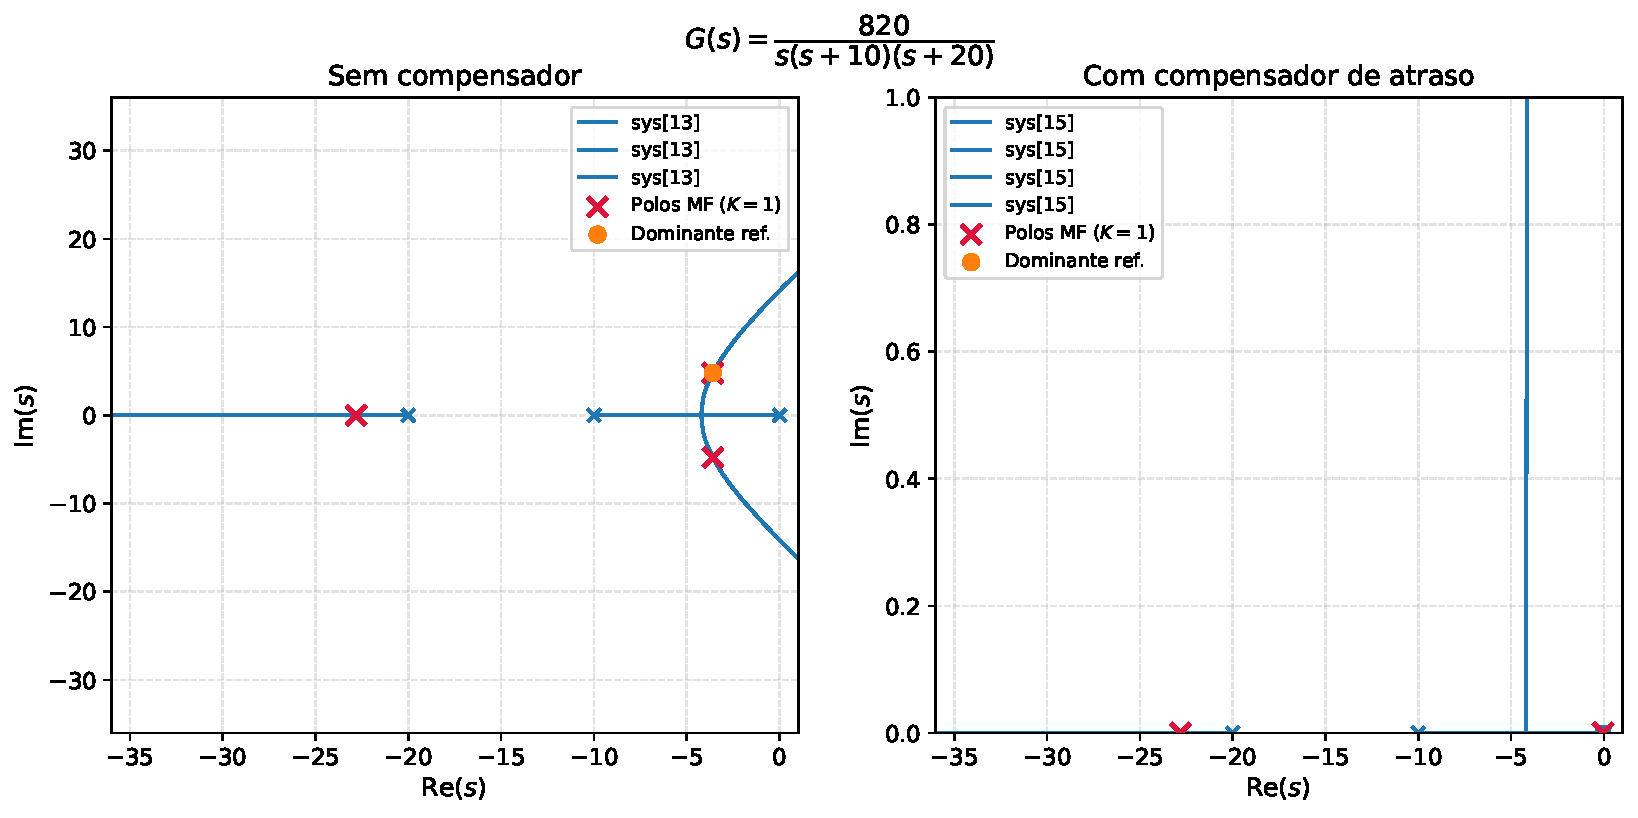
\includegraphics[width=\linewidth]{fig_b620_lugar_raizes.pdf}
  \caption{B.6.20 --- Lugar das raízes sem e com compensador de atraso; referência aos polos dominantes originais.}
  \label{fig:b620rl}
\end{figure}

\begin{figure}[htbp]
  \centering
  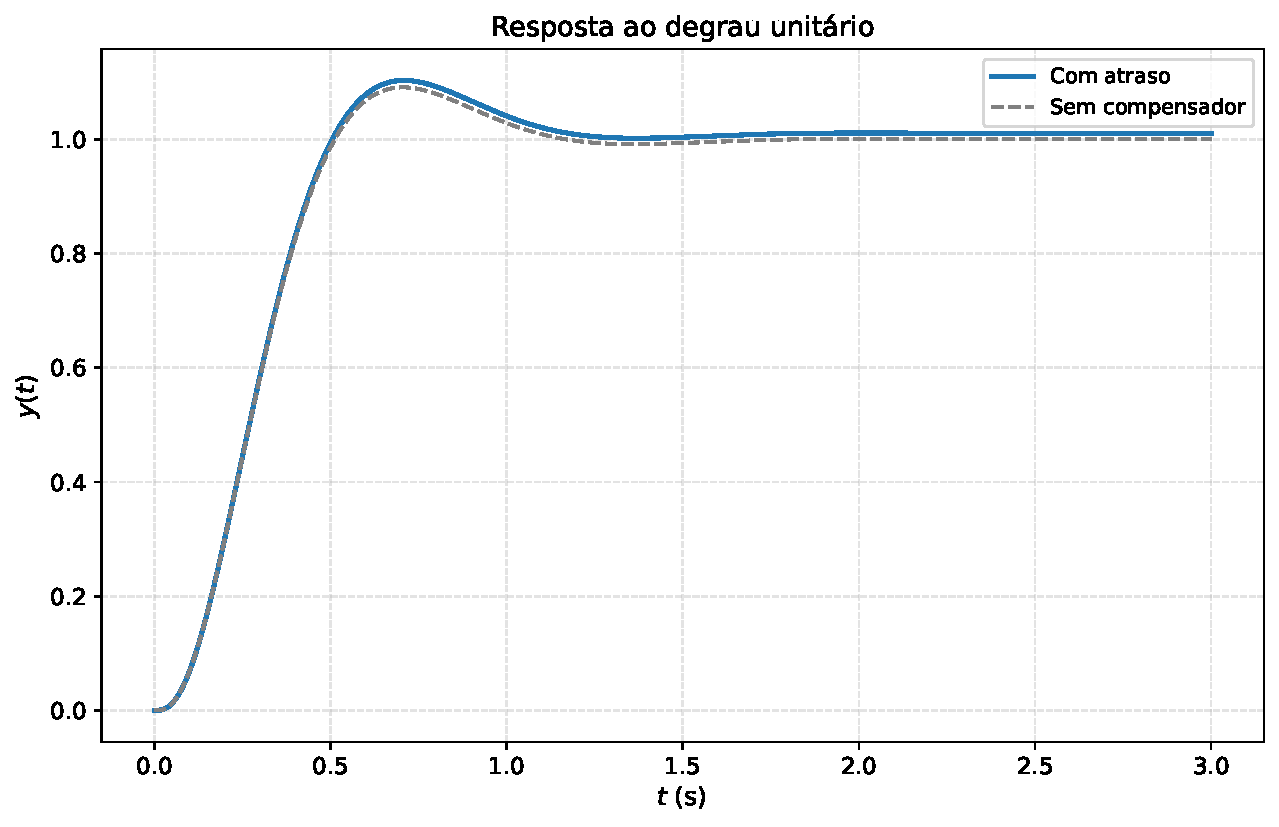
\includegraphics[width=0.92\linewidth]{fig_b620_degrau.pdf}
  \caption{B.6.20 --- Resposta ao degrau unitário com e sem compensador de atraso.}
  \label{fig:b620step}
\end{figure}

\end{document}
